\documentclass[journal, a4paper]{IEEEtran}
\usepackage{booktabs}
\usepackage{graphicx}
\usepackage{stfloats}
\usepackage{placeins}
\usepackage{url}
\usepackage{amsmath}
\usepackage{amssymb}
\interdisplaylinepenalty=2500
\newcommand{\RR}{\mathbb R}
\newcommand{\dd}{\,\mathrm d}
\newcommand{\norm}[1]{\left\lVert#1\right\rVert}
\newcommand{\cross}{\mathbin{\times}}
\begin{document}
\title{Orbit-to-Orbit PMP Candidates Across Multiple Spheres of Influence With Constant-Power, Variable-$I_{\!sp}$ Propulsion}
\author{Jan~Ol\v{s}ina\\[1ex] Independent Researcher, Prague, Czech Republic\\
email: \texttt{jan.olsina@gmail.com}, ORCID: \texttt{0009-0003-9816-3958}.}
\maketitle
\begin{abstract}
We formulate a multiphase optimal-control problem for minimum-duration orbit-to-orbit flight through a hierarchy of moving spheres of influence. The vehicle supplies constant useful jet power while powered and varies exhaust speed and thrust direction. For the ideal uncapped engine, inverse mass converts propellant expenditure into a single additive quadratic acceleration budget. We give the state and adjoint equations, moving-orbit endpoint transversality, moving-interface corner conditions, and their equivalent expressions in translating body-centred frames. In particular, regular optimal crossings preserve the physical thrust-acceleration vector, although the position costate and thrust jerk can jump. This necessary matching condition does not impose constant acceleration on an entire capture spiral. A separate numerical section describes topology enumeration, sparse multiple shooting, direct-to-indirect initialization, continuation, precomputed phase maps, and symmetry reductions, explicitly separating exact reductions from heuristic restrictions. A numerical comparison with a reoptimized constant-acceleration spiral-and-staging family illustrates thrust modulation and the cost of restricted local legs. Finally, a state-independent exhaust-speed control gives a consistent PMP for a finite specific-impulse band, including coast, upper-exhaust-speed, interior, and lower-exhaust-speed modes. These equations generate PMP candidates; they do not by themselves certify local or global optimality.
\end{abstract}

\section{Scope and conventions}
The objective is elapsed flight time $t_f-t_0$ at a specified initial mass $m_0$ and permitted propellant expenditure. Let $m_*>0$ denote the minimum allowed mass, including dry hardware and any required reserve. The constraints are $m(t)\ge m_*$ and $m(t_0)=m_0$. Unless stated otherwise, the useful jet power $P>0$ is the same in every phase, there is no staging or refuelling, and the vehicle is a point mass. Engine-off motion is allowed. The problem is nonrelativistic and excludes atmospheric braking and impulses.

We use the \emph{maximization} PMP convention
\begin{equation}
 H=p^T f-\lambda_0,\qquad \lambda_0=1
 \label{eq:convention}
\end{equation}
for normal minimum-time extremals. Costates maximize $H$ over the control set and satisfy $\dot p=-H_x$. Abnormal candidates have $\lambda_0=0$ and require separate treatment; normality is not claimed for every degenerate endpoint or active-constraint configuration. Superscripts $-$ and $+$ denote one-sided values at a transition. All equations are dimensional unless explicitly normalized.

The word ``exact'' below means exact for the \emph{specified patched gravitational model}. A sphere of influence (SOI) is a modelling boundary, not a physical discontinuity in gravity. The corresponding smooth many-body problem is a different model. General hybrid maximum/minimum principles supply the framework for the corner conditions \cite{pakniyat,pakniyat2024}.

\section{Specify the gravity model before optimizing}
\subsection{Body ephemerides and phase domains}
For each body $j$, prescribe an inertial ephemeris $\mathbf R_j(t)$, gravitational parameter $\mu_j$, and SOI radius $s_j(t)$. A candidate route has a finite sequence of active centres
\begin{equation}
 j_1,j_2,\ldots,j_N,\qquad
 t_0<t_1<\cdots<t_N=t_f.
\end{equation}
For example, moon--planet--star--planet--moon has five centre phases, not necessarily five engine modes. The centre selection rule must be specified in overlapping or nested SOIs, for example the deepest enclosing body in a fixed hierarchy. Each phase must remain in its assigned domain and cross each declared interface in the required direction. Merely solving endpoint equalities does not ensure this.

An interface for entry to or exit from body $k$ can be written
\begin{equation}
 \phi(\mathbf r,t)=\norm{\mathbf r-\mathbf R_k(t)}-s_k(t)=0.
 \label{eq:surface}
\end{equation}
At the crossing,
\begin{equation}
 \phi_{\mathbf r}=\mathbf n^T,\quad
 \phi_t=-\mathbf n\cdot\dot{\mathbf R}_k-\dot s_k,\quad
 d=\phi_t+\mathbf n\cdot\mathbf v.
 \label{eq:crossrate}
\end{equation}
Require $d<0$ for entry and $d>0$ for exit. The regular formulas assume $d\ne0$; grazing contacts and simultaneous interfaces need a distinct active-set treatment.

\subsection{A consistent common-frame realization of local Kepler phases}
The usual local two-body patch is
\begin{equation}
 \ddot{\boldsymbol\rho}_j=-\mu_j\boldsymbol\rho_j/\rho_j^3+\mathbf a,
 \qquad \boldsymbol\rho_j=\mathbf r-\mathbf R_j(t).
 \label{eq:localgravity}
\end{equation}
Its equivalent common-inertial-frame field is
\begin{equation}
 \boxed{\mathbf g_j(\mathbf r,t)=\ddot{\mathbf R}_j(t)
       -\mu_j\frac{\mathbf r-\mathbf R_j(t)}{\norm{\mathbf r-\mathbf R_j(t)}^3}.}
 \label{eq:globalgravity}
\end{equation}
The origin acceleration must not be accidentally omitted when converting between these two descriptions. Alternatively, one can deliberately define $\mathbf g_j=-\mu_j(\mathbf r-\mathbf R_j)/\rho_j^3$ in inertial coordinates; then its local equation contains $-\ddot{\mathbf R}_j$. That is a different patching approximation.

Thus changing SOI changes more than $\mu$: it changes the force centre, its ephemeris and frame translation, the phase domain, and possibly the time dependence of the field. Rotating local axes additionally introduce Coriolis, centrifugal and Euler terms. We use translating, \emph{nonrotating} axes to avoid them.

For \eqref{eq:globalgravity}, the spatial gravity Jacobian is symmetric:
\begin{equation}
 G_j=D_{\mathbf r}\mathbf g_j=
 \frac{\mu_j}{\rho_j^3}(3\hat{\boldsymbol\rho}_j\hat{\boldsymbol\rho}_j^T-I).
 \label{eq:gravityjac}
\end{equation}
A smooth many-body model can replace $\mathbf g_j$ throughout the following equations. If a phase division is then only bookkeeping, there is no physical corner or costate jump at that division.

\section{Ideal uncapped engine: one global resource}
The engine equations imply
\begin{equation}
 \dot m=-\frac{m^2\norm{\mathbf a}^2}{2P},\qquad
 B=2P\left(\frac1{m_*}-\frac1{m_0}\right).
\end{equation}
Introduce spent effort $c$ with
\begin{equation}
 \dot c=\norm{\mathbf a}^2,\quad c(t_0)=0,\quad c(t_f)\le B.
 \label{eq:effort}
\end{equation}
This is exactly the mass constraint, since
\begin{equation}
 m(t)=\left[\frac1{m_0}+\frac{c(t)}{2P}\right]^{-1}.
 \label{eq:massrecover}
\end{equation}
The budget is shared by \emph{all} phases, not reset on entering another SOI. Its units are $\mathrm{m^2\,s^{-3}}$. In the ideal model, positive fuel reserve permits any finite acceleration, with the integral constraint above. Impulsive velocity jumps have infinite quadratic effort and are not included.

Let $\eta\ge0$ be the terminal multiplier of $c(t_f)-B\le0$. The effort costate in the maximization convention is $p_c=-\eta$ and is constant. On a normal resource-binding branch with $\eta>0$,
\begin{equation}
 H_j=\mathbf p_r\cdot\mathbf v+
 \mathbf p_v\cdot(\mathbf g_j+\mathbf a)-\eta\norm{\mathbf a}^2-1.
\end{equation}
The exact phase equations are
\begin{align}
 \dot{\mathbf r}&=\mathbf v,&\dot{\mathbf v}&=\mathbf g_j+\mathbf a,\nonumber\\
 \dot{\mathbf p}_r&=-G_j^T\mathbf p_v,&
 \dot{\mathbf p}_v&=-\mathbf p_r,\label{eq:canonical}\\
 \mathbf a&=\boxed{\frac{\mathbf p_v}{2\eta}},&\dot c&=\norm{\mathbf a}^2.\nonumber
\end{align}
The inequality has complementarity $\eta[c(t_f)-B]=0$. Do not assume equality for an already-completed or otherwise degenerate problem. The ideal finite-control regular branch is the one with positive $\eta$.

\subsection{Primer acceleration variables}
Set $k=1/(2\eta)>0$, $\mathbf a=k\mathbf p_v$, and $\mathbf j=\dot{\mathbf a}=-k\mathbf p_r$. Then
\begin{equation}
 \boxed{
 \begin{aligned}
 \dot{\mathbf r}&=\mathbf v, &\dot{\mathbf v}&=\mathbf g_j+\mathbf a,\\
 \dot{\mathbf a}&=\mathbf j, &\dot{\mathbf j}&=G_j^T\mathbf a,\\
 \dot c&=\norm{\mathbf a}^2.
 \end{aligned}}
 \label{eq:primer}
\end{equation}
These are 13 scalar equations in three dimensions or nine in a planar problem. Mass is reconstructed, not shot independently. Define
\begin{equation}
 h_j=-\mathbf j\cdot\mathbf v+\mathbf a\cdot\mathbf g_j+
           \tfrac12\norm{\mathbf a}^2,
 \qquad H_j=h_j/k-1.
 \label{eq:h}
\end{equation}
In a genuinely autonomous phase $h_j$ is constant. In the common time-dependent frame,
\begin{equation}
 \dot H_j=\mathbf p_v\cdot\partial_t\mathbf g_j,
 \qquad \dot h_j=\mathbf a\cdot\partial_t\mathbf g_j.
\end{equation}
Do \emph{not} impose $H_j=0$ in every phase merely because final time is free: moving endpoints and time-dependent ephemerides alter transversality.

\section{Exact SOI stitching in a common inertial frame}
There is no physical state reset at an ideal SOI crossing:
\begin{equation}
 (\mathbf r,\mathbf v,c)^+=(\mathbf r,\mathbf v,c)^-.
 \label{eq:statejoin}
\end{equation}
Let $\nu$ be an interface multiplier, with the following sign convention. The hybrid corner conditions are
\begin{align}
 \mathbf p_r^-&=\mathbf p_r^++\nu\mathbf n,\nonumber\\
 \mathbf p_v^-&=\mathbf p_v^+,\qquad \eta^- =\eta^+,\label{eq:costatejoin}\\
 H^-&=H^+-\nu\phi_t.\nonumber
\end{align}
They include both the restriction to the crossing surface and the freely variable crossing time. In particular,
\begin{equation}
 \boxed{\mathbf a^+=\mathbf a^-.}
 \label{eq:acont}
\end{equation}
This is continuity of the physical \emph{vector} thrust acceleration, not merely its magnitude, and not continuity of total acceleration $\mathbf g+\mathbf a$.

For a transverse crossing, the multiplier can be eliminated. Write $\Delta\mathbf g=\mathbf g^- -\mathbf g^+$ and $d$ as in \eqref{eq:crossrate}. Then
\begin{equation}
 \nu=-\frac{\mathbf p_v\cdot\Delta\mathbf g}{d}.
\end{equation}
With $\zeta=k\nu$, the primer jump is
\begin{equation}
 \boxed{\zeta=-\frac{\mathbf a\cdot\Delta\mathbf g}{d},\quad
 \mathbf a^+=\mathbf a^-,\quad
 \mathbf j^+=\mathbf j^-+\zeta\mathbf n.}
 \label{eq:primerjump}
\end{equation}
Equivalently $h^- -h^+=-\zeta\phi_t$. The denominator explains the poor conditioning near grazing transitions. Eliminating $\nu$ is optional; keeping it as a multiple-shooting unknown is often safer.

If the same smooth field is used on both sides, $\Delta\mathbf g=0$, so a transverse artificial split has $\nu=0$ and continuous costates. Conversely, a discontinuous gravitational patch can produce a jerk jump while preserving thrust. None of these necessary conditions proves global optimality or says that thrust must remain constant within a phase.

\subsection{Equivalent stitching in body-centred frames}
In phase $i$ use $\boldsymbol\rho_i=\mathbf r-\mathbf R_i$ and $\mathbf w_i=\mathbf v-\dot{\mathbf R}_i$. Switching to $j$ requires
\begin{align}
 \boldsymbol\rho_j^+&=\boldsymbol\rho_i^-+\mathbf R_i-\mathbf R_j,\nonumber\\
 \mathbf w_j^+&=\mathbf w_i^-+\dot{\mathbf R}_i-\dot{\mathbf R}_j.
 \label{eq:localreset}
\end{align}
Mass or effort is unchanged. Positions and velocities expressed in different local frames are not numerically continuous.

More generally let $x^+=\mathcal R(x^-,t_s)$ be a coordinate reset and $\phi(x^-,t_s)=0$. With no switching cost,
\begin{align}
 p^-&=\mathcal R_x^T p^++\nu\phi_x,\label{eq:resetp}\\
 H^-&=H^+-p^+\cdot\mathcal R_t-\nu\phi_t.
 \label{eq:resetH}
\end{align}
For \eqref{eq:localreset}, $\mathcal R_x=I$ and
\begin{equation}
 \mathcal R_t=(\dot{\mathbf R}_i-\dot{\mathbf R}_j,
                   \ddot{\mathbf R}_i-\ddot{\mathbf R}_j,0).
\end{equation}
The last zero is the mass or effort component. The surface derivatives in \eqref{eq:resetp}--\eqref{eq:resetH} must be taken in the \emph{old local coordinates}. These formulas include the translation terms often lost by matching only $\mu$.

Local Hamiltonians obey
\begin{equation}
 H_{\rm local}=H_{\rm inertial}
       -\mathbf p_r\cdot\dot{\mathbf R}_j
       -\mathbf p_v\cdot\ddot{\mathbf R}_j.
\end{equation}
Use either the common-frame equations or the reset equations consistently; do not apply both jumps to the same interface.

\section{Orbit-to-orbit endpoint conditions}
\subsection{Circular orbit manifolds}
Fix orthonormal vectors $\mathbf e_1,\mathbf e_2$ spanning the desired orbital plane, radius $R$, and orientation sign $\sigma=\pm1$. Put
\begin{align}
 \mathbf q(\theta)&=\mathbf e_1\cos\theta+\mathbf e_2\sin\theta,\nonumber\\
 \mathbf t(\theta)&=-\mathbf e_1\sin\theta+\mathbf e_2\cos\theta.
\end{align}
The allowed orbit states about body $j$ are
\begin{equation}
 X_j(t,\theta)=
 \begin{pmatrix}
 \mathbf R_j(t)+R\mathbf q(\theta)\\
 \dot{\mathbf R}_j(t)+\sigma\sqrt{\mu_j/R}\,\mathbf t(\theta)
 \end{pmatrix}.
 \label{eq:orbit}
\end{equation}
Use separate planes and radii at departure and arrival. An elliptic orbit can replace this parameterization by its Kepler position and velocity map. If plane orientation is also free, its parameters generate additional tangent transversality equations.

Impose $(\mathbf r,\mathbf v)(t_0)=X_D(t_0,\theta_0)$ and $(\mathbf r,\mathbf v)(t_f)=X_A(t_f,\theta_f)$. For each free endpoint phase,
\begin{equation}
 p_{rv}(t_0)\cdot X_{D,\theta}=0,\qquad
 p_{rv}(t_f)\cdot X_{A,\theta}=0,
 \label{eq:phaseend}
\end{equation}
where $p_{rv}=(\mathbf p_r,\mathbf p_v)$. In primer variables this is
\begin{equation}
 -\mathbf j\cdot X_{\theta,r}+\mathbf a\cdot X_{\theta,v}=0.
\end{equation}
Omit the departure equation if departure state/phase is fixed. A free phase at a chosen epoch is an assumption, not permission to teleport an actual parked ship. For an actual known initial phase, either propagate it to the chosen departure epoch or include an explicit waiting phase.

\subsection{Free final time, launch date, and fuel}
For free $t_f$ and target \eqref{eq:orbit},
\begin{equation}
 \boxed{H(t_f)-p_{rv}(t_f)\cdot X_{A,t}(t_f,\theta_f)=0.}
 \label{eq:tf}
\end{equation}
Here the partial derivative holds the free phase parameter fixed. In ideal primer variables,
\begin{equation}
 h(t_f)-k+\mathbf j(t_f)\cdot X_{A,t,r}
              -\mathbf a(t_f)\cdot X_{A,t,v}=0.
 \label{eq:tfprimer}
\end{equation}
If the target is stationary as a phase-space manifold, this reduces to $H(t_f)=0$. For a particular moving station, replace the manifold by its full ephemeris, omit free-phase transversality, and differentiate the station state with time.

For a free interior departure date minimizing \emph{flight duration}, there is also
\begin{equation}
 H(t_0)-p_{rv}(t_0)\cdot X_{D,t}=0.
 \label{eq:t0}
\end{equation}
At launch-window endpoints use one-sided KKT conditions. Minimizing arrival epoch from a fixed current epoch, including waiting, is a different objective; a fixed-start waiting phase is a straightforward formulation. It must not be silently identified with minimizing flight duration over an unrestricted launch date.

The ideal terminal resource conditions are $c_f\le B$, $\eta\ge0$, and $\eta(c_f-B)=0$. For the original mass formulation used below, they are
\begin{equation}
 m_f\ge m_*,\quad p_m(t_f)=\kappa\ge0,\quad
 \kappa(m_f-m_*)=0,
 \label{eq:massend}
\end{equation}
provided no additional mass-dependent terminal objective or constraint is present. Initial mass is fixed and has no prescribed initial costate. Binding-terminal-fuel candidates satisfy $m_f=m_*$. In the ideal interior model $p_m m^2=2P\eta$, consistently relating the two formulations.

\section{The complete candidate boundary-value problem}
For each specified centre itinerary, the unknowns are phase-interface states and costates, positive phase durations, the free endpoint phases and dates, interface multipliers, and a resource multiplier. Solve simultaneously:
\begin{enumerate}
\item The phase ODEs \eqref{eq:canonical} or \eqref{eq:primer}.
\item Position, velocity and effort/mass stitching, plus each SOI equation and correct crossing direction.
\item Costate and Hamiltonian corner conditions \eqref{eq:costatejoin}, or their local reset equivalents.
\item Endpoint orbit membership, free-phase transversality, final-time transversality, and resource complementarity.
\item Any imposed launch-window and path-constraint conditions.
\end{enumerate}
There is only one global effort budget and one ideal resource multiplier. Do not impose a fresh $H=0$ or choose an independent costate scale for each patch. Do not prescribe circular states at intermediate staging radii unless these are genuine mission requirements. Such restrictions solve a smaller feasible problem.

Necessary path constraints include exclusion of physical bodies, correct phase-domain membership, and any thermal or operational limits. The displayed smooth-arc PMP applies where those inequalities are inactive. If an optimum touches a path boundary, it requires the corresponding state-constraint multipliers and boundary-arc equations. A direct constrained transcription can discover that active set before an indirect refinement. Rejecting all such candidates is a declared restriction, not an exact solution of the original constrained problem.

\subsection{A concrete residual count for implementation}
For a fixed initial position, velocity and epoch, a phase-free circular target in a fixed plane, binding fuel, and no active path constraints, a three-dimensional single-shooting parameter vector can be
\begin{equation}
 Z=(\mathbf a_0,\mathbf j_0,k,t_f,\theta_f,
             \{t_i,\zeta_i\}_{i=1}^{N-1}).
\end{equation}
It has $9+2(N-1)$ scalar unknowns. Start from the prescribed physical state and $c_0=0$, integrate each primer phase to its proposed $t_i$, and apply $\mathbf j^+=\mathbf j^-+\zeta_i\mathbf n_i$, with $\mathbf r,\mathbf v,\mathbf a,c$ continuous. At each interface retain the two residuals
\begin{equation}
 \phi_i=0,\qquad h_i^- -h_i^+ +\zeta_i\phi_{i,t}=0.
\end{equation}
The nine final residuals are six orbit-state matching equations, one free-phase condition, one free-time condition \eqref{eq:tfprimer}, and $c_f-B=0$. Enforce $k>0$, ordered times and correct crossing directions. This gives a square normal-candidate system. Multiple shooting expands this system by introducing segment initial values and matching equations without changing its content.

A free departure phase adds one unknown and its transversality equation; a free departure date adds one unknown and \eqref{eq:t0}, subject to launch-window KKT conditions. A fixed arrival phase removes its unknown and phase-transversality equation. In a strictly planar problem replace the six initial primer components and six endpoint state residuals by four each, giving $7+2(N-1)$ unknowns and residuals for the otherwise identical setup. These counts apply to the stated endpoint freedoms, not to an arbitrary mixture of orbit and rendezvous constraints.

\section{Exact reductions and reusable calculations}
This section describes operations that preserve the specified model; the next section contains search heuristics.

\subsection{Scaling and trajectory reuse}
For a local Kepler phase with reference radius $L$,
\begin{align}
 t_K&=\sqrt{L^3/\mu}, &v_K&=\sqrt{\mu/L},\nonumber\\
 a_K&=\mu/L^2, & B_K&=\mu^{3/2}/L^{5/2}.
\end{align}
Use consistent scales for states, costates, interface residuals and durations. In separate phase units, first unscale to physical quantities before matching, or include all scale factors in the reset Jacobian. Equating dimensionless acceleration values from different phase scales is generally wrong.

The ideal dynamics and fixed-time minimum effort depend on the ship only through the final comparison with $B$. Dimensionless phase solution families and their sensitivities can therefore be reused across ships, provided the boundary geometry and constraints are included in the family parameters. A finite exhaust band destroys this one-budget ship independence.

\subsection{Local symmetries and phase elimination}
For autonomous central gravity, the primer equations conserve
\begin{equation}
 \mathbf K=\boldsymbol\rho\cross\mathbf j-\mathbf w\cross\mathbf a.
\end{equation}
In a planar terminal capture phase with free circular-orbit arrival phase, the relevant scalar $K$ is zero. The angle can then be removed exactly. Writing $u=v_r$, $w=v_\theta$, $\alpha=a_r$, $\beta=a_\theta$, and $q=-(\dot{\mathbf a})_r$ gives
\begin{align}
 \dot r&=u,\qquad \dot u=w^2/r-\mu/r^2+\alpha,\nonumber\\
 \dot w&=-uw/r+\beta,\nonumber\\
 \dot\alpha&=-q+w\beta/r,\nonumber\\
 \dot\beta&=-2w\alpha/r+u\beta/r,\label{eq:reduced}\\
 \dot q&=\alpha(w^2/r^2-2\mu/r^3)-\beta uw/r^2.\nonumber
\end{align}
Add $\dot c=\alpha^2+\beta^2$ and recover $\theta$ by quadrature. This reduction is useful for a phase-free terminal capture map. It cannot be indiscriminately applied to an intermediate moon encounter: subsequent geometry usually breaks the free-phase condition. In three dimensions, a fixed target plane leaves less symmetry; do not set all three components of $\mathbf K$ to zero merely because orbital phase is free.

\subsection{Variational equations and interface sensitivities}
Integrate state/costate transition matrices or automatic-differentiation sensitivities together with each segment. The Kepler gravity Jacobian \eqref{eq:gravityjac} is analytic. Cache endpoint maps and their Jacobians for repeated local geometries; retain branch identifiers and validity ranges.

For event-driven state propagation through an identity-reset surface, the state saltation matrix is
\begin{equation}
 S=I+\frac{(f^+-f^-)\phi_x}{\phi_t+\phi_x f^-}.
 \label{eq:saltation}
\end{equation}
It maps perturbations compared at the same nominal time and accounts for the shifted event time. The adjoint jump is consistent with $p^-=S^Tp^+$ for this identity-reset event. For full state--costate propagation, differentiate the full event map, including the multiplier and its jump; applying only the physical-state matrix to every variable is insufficient. An alternative is explicit interface nodes and times, differentiating the surface and matching residuals directly. This often avoids fragile event-time derivatives near grazing.

\subsection{Fixed-time effort subproblems and exact gradients}
For the ideal engine one can first solve the fixed-$T$ minimum-effort problem and then seek the earliest $T$ with $J_{\min}(T)\le B$. On a smooth extremal branch,
\begin{equation}
 \delta J=\left[-2\mathbf j\cdot\delta\mathbf r+
     2\mathbf a\cdot\delta\mathbf v-2h\,\delta t\right]_{t_0}^{t_f}
 \label{eq:gradient}
\end{equation}
within a phase. Sum these contributions and enforce interface constraints to obtain whole-route derivatives. This retains the influence of changing interface positions and velocities, which an endpoint-acceleration-only rule misses.

For an isolated phase-free circular target, a captured craft can coast on the orbit, so the global exact-duration effort value is nonincreasing with allowed duration. A restricted revolution branch need not have that property. For moving or otherwise constrained targets and routes, establish any monotonicity used by a root search rather than assuming it. The first feasible crossing of one branch is not necessarily the first crossing of all branches.

\section{Numerical search strategy and heuristics}
The following is a practical strategy, not a proof that all PMP candidates are found.

\subsection{Outer discrete search}
Enumerate plausible centre itineraries, launch-date windows, prograde/retrograde choices, and revolution or encounter branches. Nested-SOI hierarchy removes impossible direct transitions. A monotonic outbound--inbound itinerary is a useful initial restriction, but flybys and reentries can improve some problems; declare them excluded if they are not searched. Revolution count is a branch label to track, not an extra equality that must be imposed on every orbit-to-orbit problem.

Precompute ephemerides and SOI radii with smooth interpolation and controlled derivative error. Coarse ballistic or Lambert transfers can rank dates and approach geometries, but rejecting a geometry solely because its ballistic seed is poor is heuristic. In an isolated Kepler phase, energy and angular momentum at an entry sphere provide informative labels; SOI position, plane, time and velocity still matter to the adjoining phase.

\subsection{Obtain feasible seeds before solving full adjoints}
Useful initial paths include the game's integrated tangential spirals, low-thrust averaged spirals, ballistic arcs with finite powered corrections, and free-space minimum-effort segments. For fixed endpoints in free space,
\begin{equation}
 J_0(T)=\frac{12}{T^3}\norm{\mathbf d-\tfrac T2(\mathbf v_i+\mathbf v_f)}^2
       +\frac{\norm{\mathbf v_f-\mathbf v_i}^2}{T}.
\end{equation}
Its acceleration is affine in time. This is an exact free-space seed, not a lower bound for a gravitational transfer. Likewise a Lambert impulse must be replaced by a finite-duration burn: impulses are inadmissible under a quadratic acceleration budget.

For a slowly changing near-circular radius, an averaged spiral has
\begin{equation}
 J_{\rm av}(T)=D^2/T,\qquad
 D=\left|\sqrt{\mu/r_f}-\sqrt{\mu/r_i}\right|.
\end{equation}
It supplies a cheap time/fuel allocation seed. It is not the exact capture value. Test small eccentricity and $4\pi ar^2/\mu\ll1$ throughout its use. An inner averaged phase plus a flexible outer approach is often a better seed than extending that law to the SOI.

A coarse direct collocation or multiple-shooting nonlinear program should first optimize interface states, controls and durations under the real endpoint constraints. Its dual variables provide approximate costates. Check their convention, scaling and mesh convergence before using them as an indirect initial guess. A single failed direct spline parameterization does not establish failure of all direct collocation methods; sparse state-control transcriptions and refinement have different conditioning.

\subsection{Sparse multiple shooting}
Subdivide long centre phases into shorter numerical segments. At an artificial segment boundary impose full state and costate continuity, with no SOI multiplier. At a physical model interface impose the actual corner conditions. Use positive duration parameterizations and scaled residuals. Assemble the block-sparse Jacobian and solve the Newton step with a trust region or line search. Condense well-conditioned short segments; retain independent nodes across strongly sensitive sections and near encounters.

Compared with single shooting, this prevents one unstable long integration from amplifying every initial-costate error. It does not eliminate nonconvexity or guarantee convergence. Use orbital-element or regularized coordinates when they improve conditioning, but nonsingular Cartesian coordinates remain preferable near elements' singularities. Any time regularization must transform the Hamiltonian and costates consistently.

\subsection{Continuation and branch tracking}
Start with an easier member of the family: longer flight time, a nearby solved route, smaller endpoint displacement, or a smoothed/modified gravity model. Continue to the required model and budget with adaptive steps. Gravity homotopy changes the physical problem until its parameter reaches one; intermediate solutions are only seeds.

Use pseudo-arclength continuation near folds rather than assuming that time or fuel is a single-valued branch parameter. Preserve several competing branches, particularly different revolution counts or periapsis geometries. Continue in launch date, budget, target radius and interface velocity as appropriate. Record failures separately from infeasibility. A cache must not interpolate blindly across branch changes or into collision regions.

For expensive capture phases, tabulate solutions as a function of entry radius, radial/tangential speed and allocated budget in normalized units. A phase-free planar capture at fixed entry-radius ratio still has a three-argument value map, not one spiral-acceleration parameter. Store endpoint gradients, winding information and residual estimates. Interpolation supplies initial guesses; re-solve and verify the chosen trajectory before treating it as feasible. Local sensitivities can optimize the interface without fully resolving every trial from a cold start.

\subsection{A concrete solve loop}
\begin{enumerate}
\item Define ephemerides, gravity convention, endpoint freedoms, fuel, SOI hierarchy, launch objective and physical exclusions.
\item Generate several itineraries and coarse dates/geometries; retrieve or construct seeds for all retained branches.
\item Solve a coarse constrained direct problem with free SOI states and times; refine until it is a useful feasible seed.
\item Convert its duals or nearby primer solutions into a scaled sparse multiphase indirect BVP. Enforce all state, costate, Hamiltonian and endpoint residuals jointly.
\item Continue to the requested budget and physical model, splitting difficult arcs and tracking folds. For a fixed-time strategy, search the earliest fuel-feasible time across retained branches.
\item Independently propagate the final control, checking physical states, fuel, domain membership, crossing directions, all active constraints and the Hamiltonian-maximization condition.
\item Compare elapsed times among verified feasible candidates. Report the best as ``best found PMP candidate'' unless a sufficient optimality test or global bound closes the gap.
\end{enumerate}
Conjugate-point or second-variation analysis can establish local sufficiency under suitable hypotheses. Global certification requires stronger comparison, such as a verified value function or matching global lower bound. Neither small shooting residuals nor many successful initial guesses alone provide it.

\section{Numerical demonstration and comparison with a spiral planner}
\label{sec:demonstration}
\subsection{Matched vehicle, gravity and boundary conditions}
The following examples use the ship in the companion manuscript \cite{companion}: useful jet power $P=1\,\mathrm{GW}$, initial mass $m_0=3\times10^6\,\mathrm{kg}$ and dry mass $m_*=10^6\,\mathrm{kg}$. Thus
\begin{equation}
 B=2P(1/m_*-1/m_0)=1333.333333\,\mathrm{m^2\,s^{-3}}.
\end{equation}
The engine is ideal and uncapped; no finite exhaust-speed band is imposed. Both methods start in a prograde circular orbit $100\,\mathrm{km}$ above the Moon and finish in a prograde circular orbit $200\,\mathrm{km}$ above Mars, with free orbital phase. They share the same prescribed coplanar ephemerides, launch instant and quadratic budget. The final propagated mass is approximately $1{,}000{,}000.067\,\mathrm{kg}$ in each case.

For the Solar-System example, Earth and Mars have circular heliocentric orbital radii $1$ and $1.523679\,\mathrm{AU}$; Mars initially leads Earth by $30^\circ$. The Moon starts $90^\circ$ from the common inertial $x$ axis at a geocentric distance of $384{,}400\,\mathrm{km}$. Angular velocities follow the stated circular-orbit model, and SOIs use $r_{\rm SOI}=a(\mu/\mu_{\rm parent})^{2/5}$. This is a specified launch geometry, not a dated ephemeris prediction. Local motion uses central gravity of the active body, with physical position and velocity matched at each moving SOI. These are the translating-centre patched equations discussed earlier, not a smooth simultaneous many-body integration.

\subsection{What the game comparison includes}
The supplied \texttt{TheLongBurn.zip} implements the local law
\begin{equation}
 \mathbf a_T=\sigma A\frac{\mathbf v_{\rm rel}}{\norm{\mathbf v_{\rm rel}}},
 \qquad \sigma=+1\ \hbox{(escape)},\quad -1\ \hbox{(capture)},
 \label{eq:game-law}
\end{equation}
in \texttt{tlb\_transfer/src/spiral.rs}; $A$ is constant and the effort is $A^2T$. Here ``tangential'' means along velocity, not necessarily the transverse polar direction on an eccentric trajectory. Capture is generated by backward integration from the final circular orbit. The planner's default arrival/departure acceleration ratio is one \cite{longburn}.

For a moon-to-another-planet transfer the planner also introduces a circular staging orbit about the departure planet. We reproduce the five-phase family: Moon escape, a flexible Earth-centred connector ending on the staging circle, constant-$A$ Earth escape, a flexible heliocentric leg, and constant-$A$ Mars capture. The staging radius is $a_M+1.5r_{{\rm SOI},M}$ when this is at most $0.8r_{{\rm SOI},E}$; the source's inner alternative applies otherwise. Here the outer choice is valid in both examples. We retain the Earth connector's two-planet-radius exclusion and its duration range of $0.01$--$1$ lunar periods.

The dashed curves are a \emph{reoptimized source-law family}: the shared $A$, spiral orientations, connector controls and transition times are optimized jointly. Reusable one-parameter spiral maps reduce this solve to two flexible legs; the selected spirals are then reintegrated directly. This is a Python reimplementation of the source's steering and staging restrictions, not a run of the Rust planner's coarse searches, phase-alignment heuristics or runtime. It is consequently a controlled comparison of trajectory families, not a benchmark of the game executable. The baseline can have thrust jumps at joins. The flexible four-phase candidate has no compulsory staging circle and permits radial and transverse thrust modulation; thrust-vector continuity is enforced at its physical SOI joins before small feasibility corrections.

\subsection{Acceleration zooms and reference frames}
Figure~\ref{fig:moonmars-comparison} adds local trajectory views, departure and arrival acceleration zooms, and a decomposition of the final capture thrust. All magnitude panels plot
\begin{equation}
 q(t)=\norm{\mathbf a_T(t)},
\end{equation}
not $\norm{\mathbf g+\mathbf a_T}$. The same physical thrust vector has the same norm in heliocentric or body-centred axes, including after a rotation of the plotting axes. A coordinate acceleration in an accelerating frame would require the inertial terms, but that is not the quantity plotted here. The radial/transverse components use the instantaneous local basis $(\mathbf e_r,\mathbf e_\theta)$ and therefore do depend on that rotating basis. The magnitude oscillations cannot be explained away by that rotation.

On a smooth unconstrained ideal PMP arc, the primer equations give
\begin{equation}
 \ddot{\mathbf a}_T=G^T\mathbf a_T,\qquad
 G=\frac{\mu}{r^3}(3\mathbf e_r\mathbf e_r^T-I).
\end{equation}
Writing the inertial direction rate of nonzero thrust as $\omega_a$ and its angle to $\mathbf e_r$ as $\gamma$ yields
\begin{equation}
 \ddot q=q\left[\omega_a^2+\frac{\mu}{r^3}(3\cos^2\gamma-1)\right].
\end{equation}
This displays the coupling of thrust modulation to the gravity gradient and changing geometry. It does not predict a universal oscillation period or prove that the finite-dimensional, feasibility-corrected trajectories exactly satisfy the continuous PMP. The plotted modulations are smooth and resolved under mesh refinement. Capture zooms align each method to its own arrival time, rather than comparing unequal physical flight phases at the same elapsed time.

\begin{figure*}[!t]
\centering
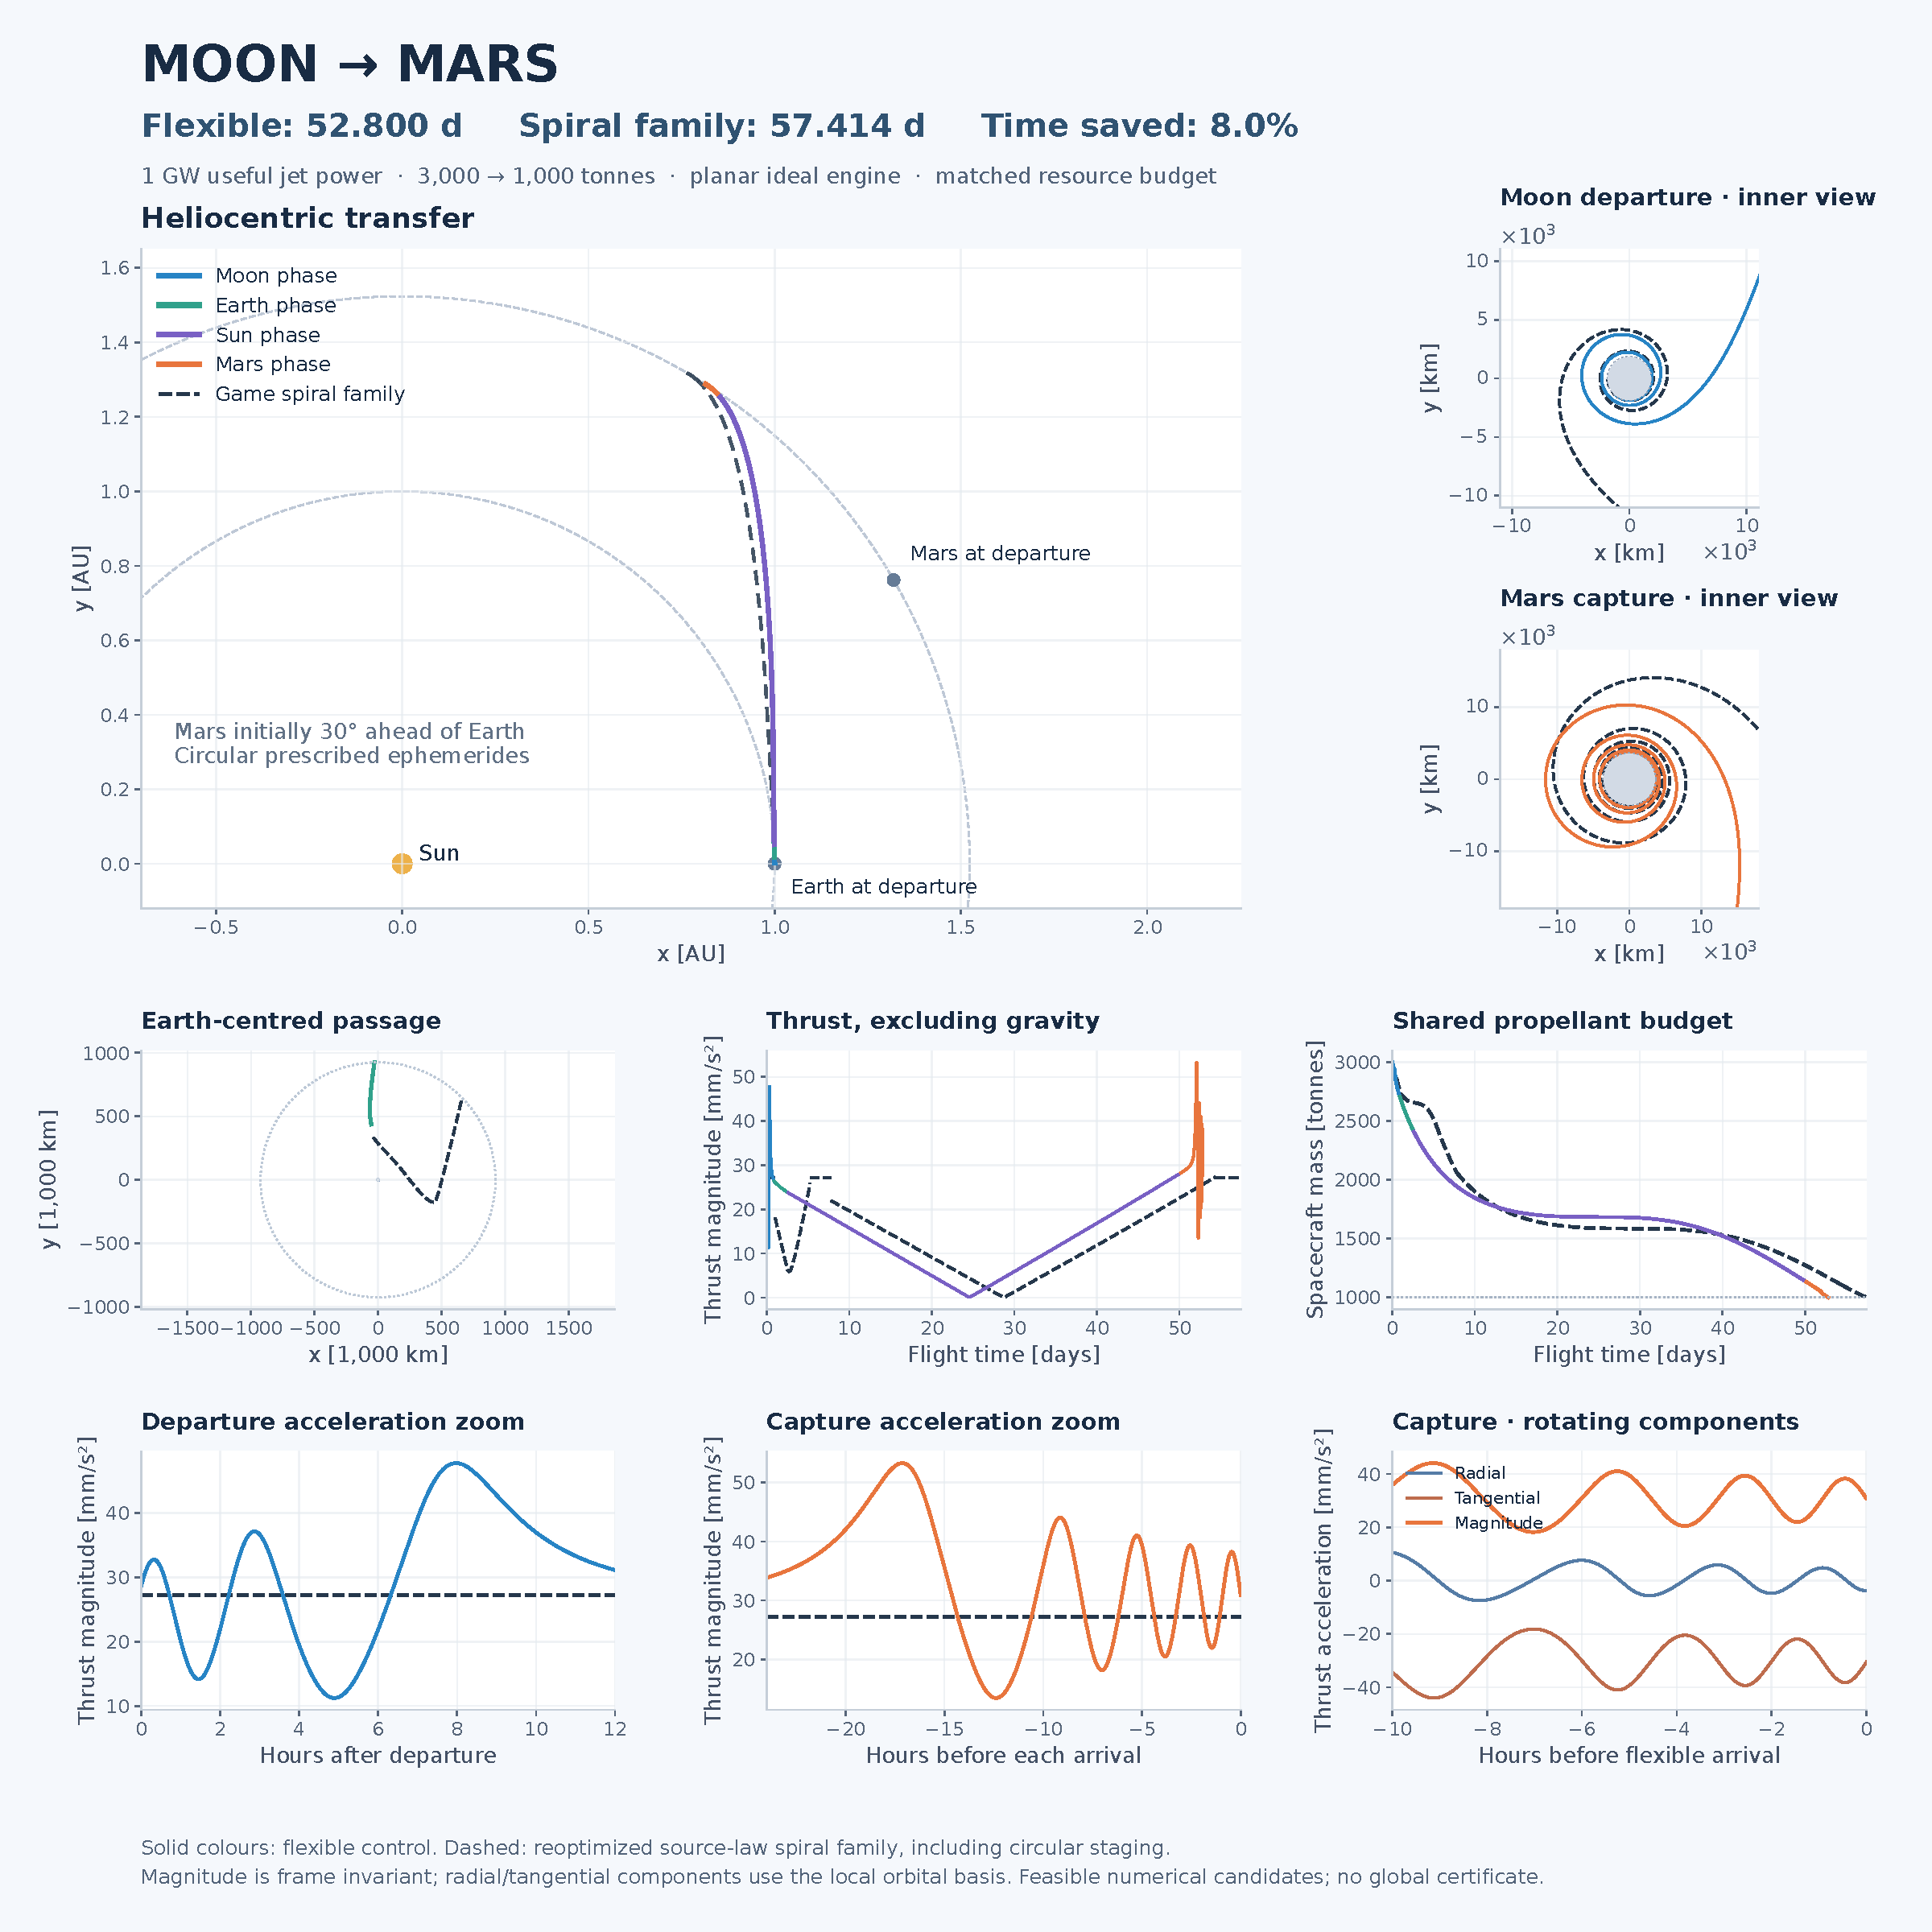
\includegraphics[width=\textwidth]{figures/moon_mars_comparison.pdf}
\caption{Matched Moon-to-Mars comparison. Solid phase colours show the flexible candidate; dashed curves show the reoptimized constant-acceleration spiral-and-staging family. The bottom row resolves the first $12$ hours of lunar departure, the last $24$ hours of Mars capture, and the last $10$ hours of capture components. The two methods choose their own free parking-orbit phases. The norm oscillations are physical thrust modulation, whereas the signed components are expressed in the rotating local orbital basis.}
\label{fig:moonmars-comparison}
\end{figure*}

\subsection{A constructed configuration with a larger gap}
To make local-leg restrictions more consequential, keep the Sun and ship unchanged and multiply each Earth, Moon and Mars analogue's mass by $s=0.003$ and radius by $s^{1/3}$ (unchanged mean density). Put the planetary analogues on circular $1$ and $1.006\,\mathrm{AU}$ orbits, initially aligned. Their heliocentric speeds are $29.7847$ and $29.6957\,\mathrm{km\,s^{-1}}$. Scale the lunar orbital radius by $s^{2/5}$ to $37{,}638.463\,\mathrm{km}$ and keep its initial phase $90^\circ$; the relative lunar speed is $179.336\,\mathrm{m\,s^{-1}}$. Keep the parking altitudes $100$ and $200\,\mathrm{km}$. This is a hypothetical prescribed-orbit system, not a claim of long-term many-body stability. Full constants are supplied with the prototype.

The resulting Moon, Earth and Mars SOI radii are $6480.290$, $90{,}536.639$ and $37{,}316.412\,\mathrm{km}$; the staging radius is $47{,}358.898\,\mathrm{km}$. Figure~\ref{fig:large-gap-comparison} uses an Earth-following corotating overview to resolve the nearby planetary orbits. Local inner views remain body-centred and the thrust magnitudes retain their physical meaning.

\begin{table}[!t]
\caption{Matched feasible-candidate durations. Saving is relative to the reoptimized spiral family, $100(1-T_{\rm flexible}/T_{\rm spiral})$.}
\label{tab:numerical-comparison}
\centering
\begin{tabular}{lrrr}
\toprule
Configuration & Flexible [d] & Spiral [d] & Saving \\
\midrule
Moon--Mars & 52.79987 & 57.41351 & $8.04\%$ \\
Scaled close planets & 2.22147 & 3.12747 & $28.97\%$ \\
\bottomrule
\end{tabular}
\end{table}

The baseline selects $A=0.027224\,\mathrm{m\,s^{-2}}$ in the Solar-System case and $0.103600\,\mathrm{m\,s^{-2}}$ in the constructed case. In the latter, the two Earth-centred baseline phases take $1.04581\,\mathrm d$, versus $0.32697\,\mathrm d$ for the flexible Earth passage. Of the total $0.90600\,\mathrm d$ improvement, $0.71884\,\mathrm d$ occurs in that part of the route. The staging detour and resource allocation are therefore central to this example; the $28.97\%$ gap must not be attributed solely to oscillating thrust magnitude or solely to steering law \eqref{eq:game-law}. The changes to steering, common acceleration and staging are not isolated by this experiment.

\begin{figure*}[!t]
\centering
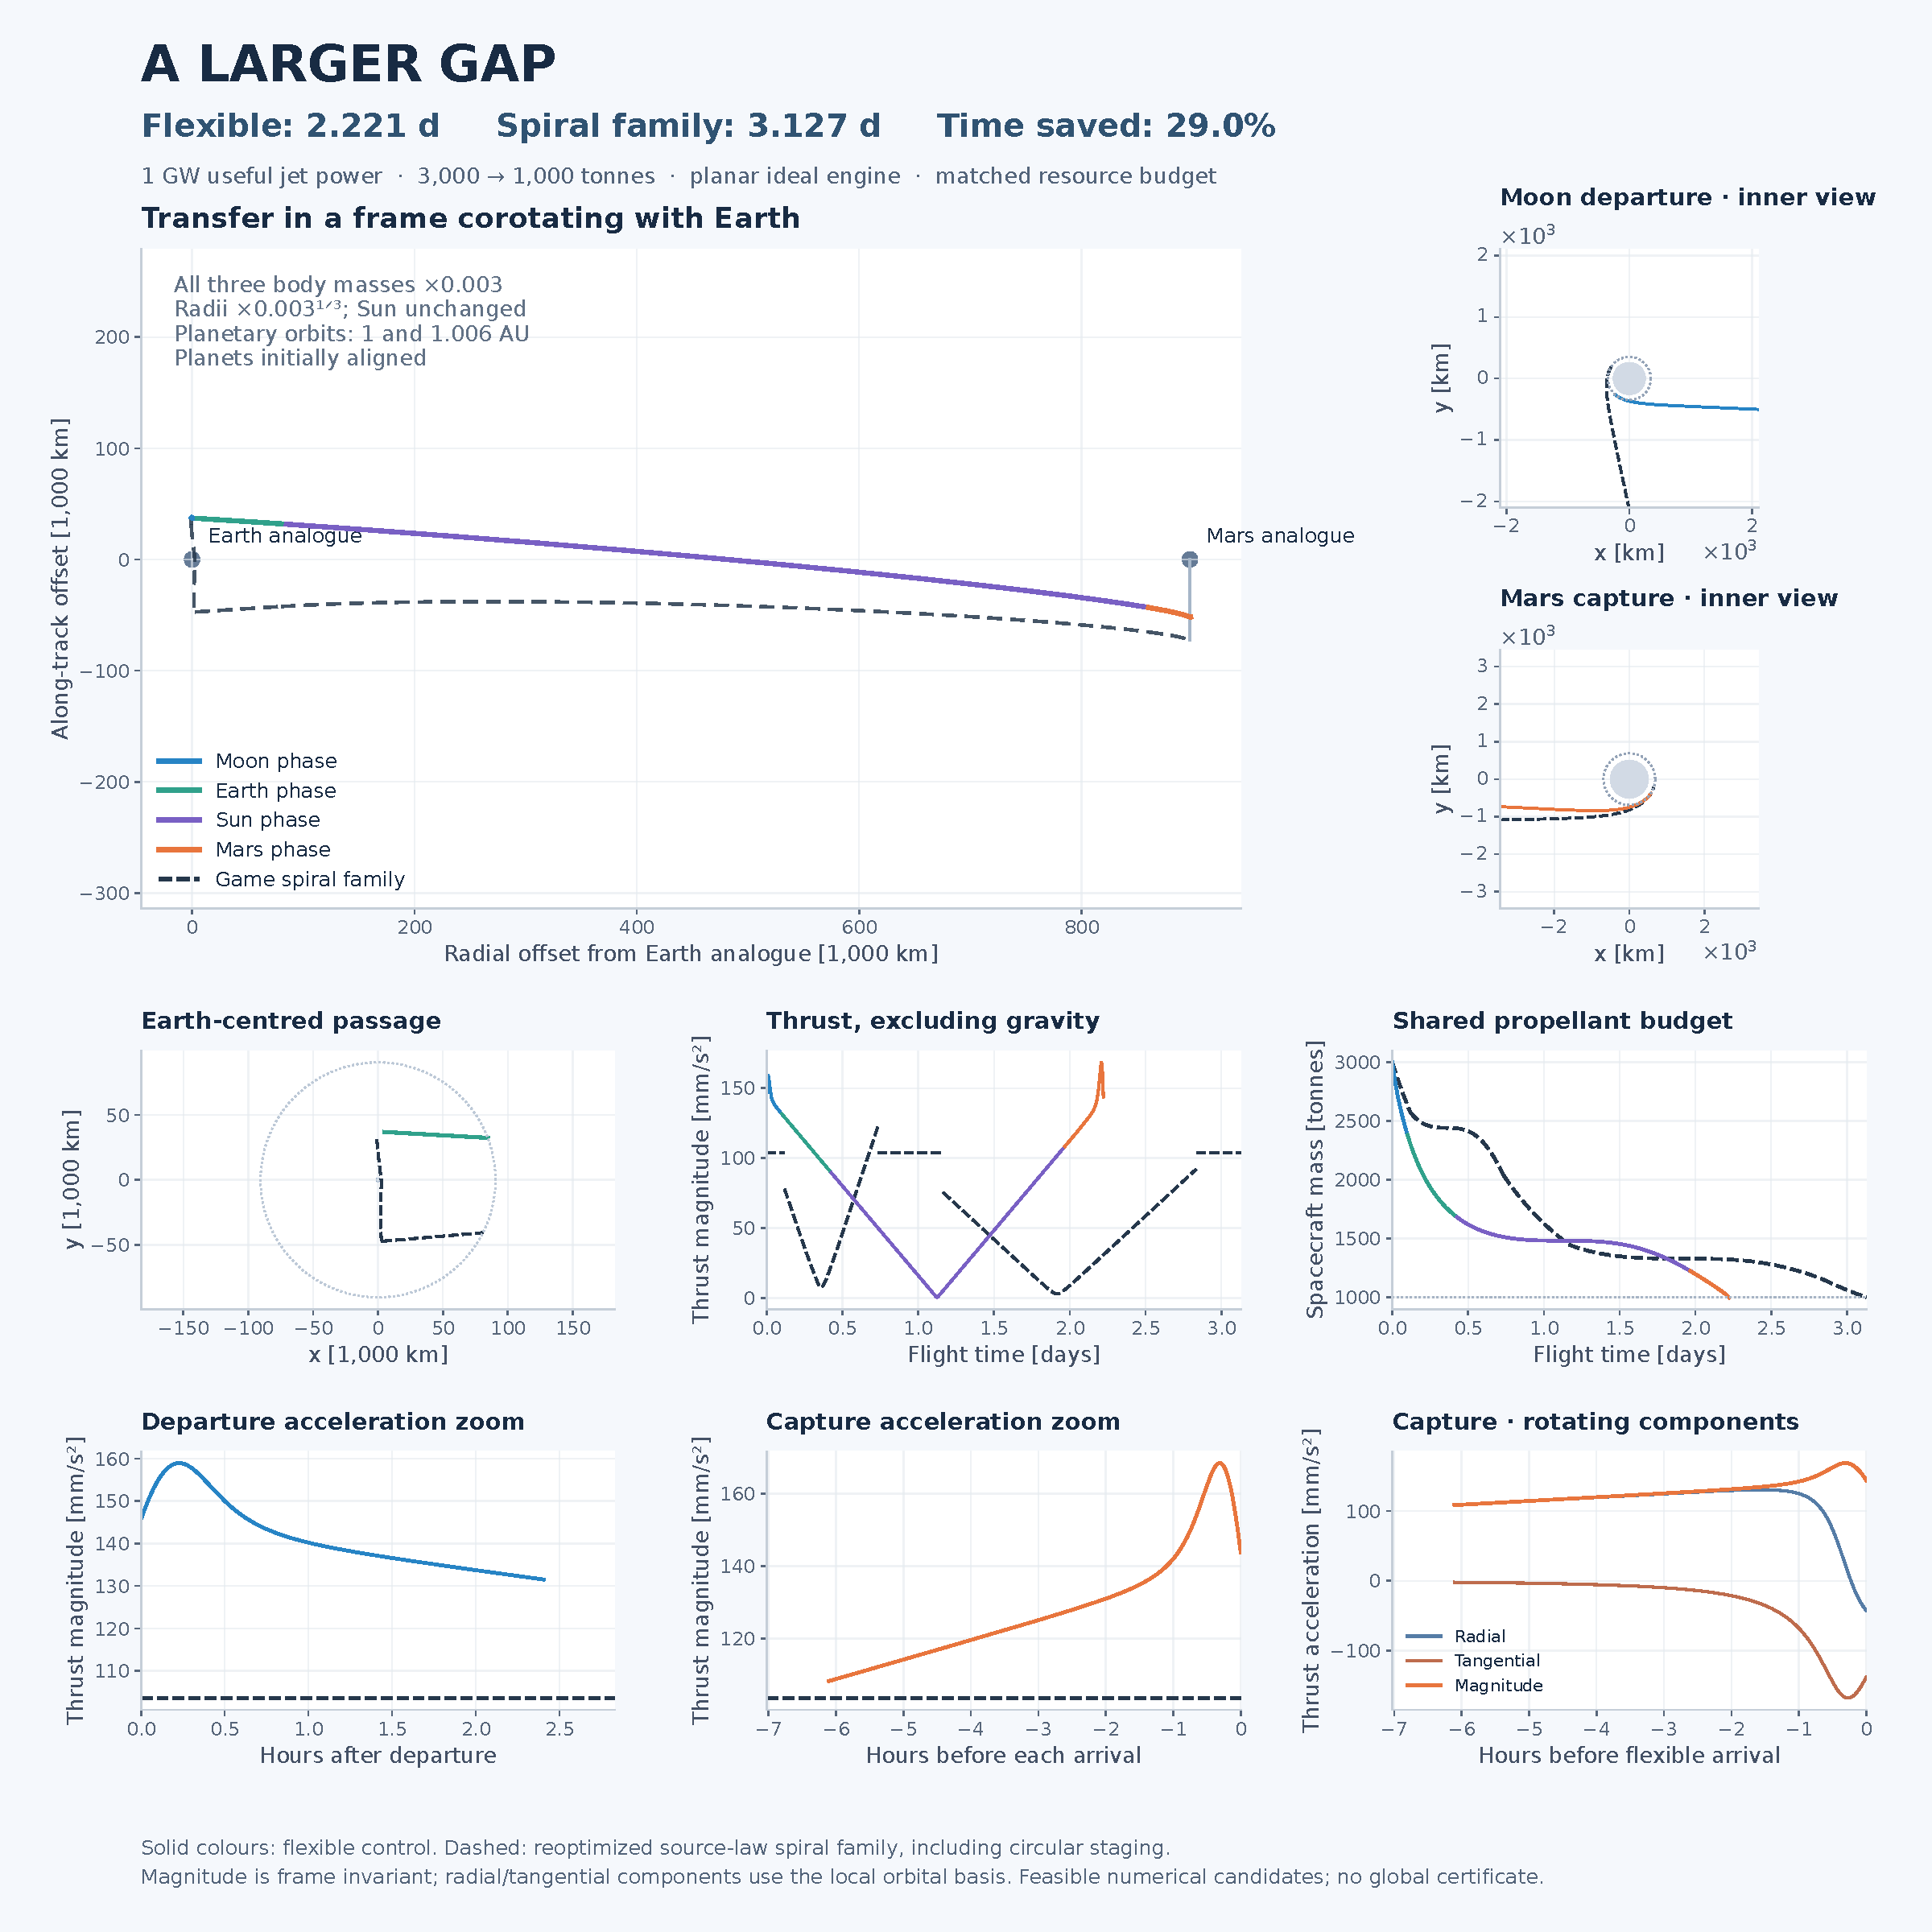
\includegraphics[width=\textwidth]{figures/large_gap_comparison.pdf}
\caption{A larger difference with the same ship in the explicitly scaled system. Nearby planetary orbits shorten the heliocentric leg and expose the cost of the staging-and-spiral restrictions. The overview is corotating; local panels are body-centred. The bottom magnitude panels cover only the respective Moon and Mars phases, aligned to departure or each method's arrival. No claim of a maximum possible performance gap is made.}
\label{fig:large-gap-comparison}
\end{figure*}

\subsection{Verification and scope of the numerical evidence}
The flexible transcription uses degree-five Radau collocation, continuous piecewise-linear local thrust components and the Sundman variable $\dd t/\dd s=r/V_{\rm ref}$. The original Moon--Mars result uses phase meshes $(300,300,160,540)$; its preceding refinement changes time by about $0.003\,\mathrm s$. The constructed case uses $(220,160,160,360)$; refinement from $(100,80,80,180)$ changes its uncorrected duration by less than $0.001\,\mathrm s$. The condensed baseline uses $(160,200)$ on its two free legs, with a refined local spiral map. Its refinement changes the uncorrected durations by less than $0.003\,\mathrm s$ in both examples.

Independent Cartesian DOP853 propagation carries the incoming state across every interface, without resetting it to an optimized endpoint. Small shooting corrections close endpoints and use the common budget, while retaining the baseline's exact constant-$A$ spiral law. The changes in flight time are approximately $-1.02$ and $-14.84\,\mathrm s$ for the Solar-System flexible and baseline candidates, and $-0.64$ and $-0.88\,\mathrm s$ for the corresponding scaled candidates. These corrections and their control changes are retained in the data. All four final checks pass: radius errors below $0.5\,\mathrm m$, radial and transverse speed errors below $0.003\,\mathrm{m\,s^{-1}}$, adequate final mass, and sampled SOI-domain and clearance checks. Small solver residuals belong to the uncorrected transcription; they are not an indirect PMP or second-variation certificate for the corrected controls.

The exploratory search tested three scaled systems. One unconverged result was rejected despite its apparently larger gap; the two converged cases gave approximately $29\%$ savings, and the larger of these was refined and plotted. Neither this search nor the two optimized trajectory families establish global optimality, a worst-case gap, or a general mission-performance guarantee. The bundle includes configurations, controls, replayed states, validation reports, refinement data and reproducible figure code.
\clearpage
\twocolumn
\setlength{\abovedisplayskip}{6pt plus 2pt minus 2pt}
\setlength{\belowdisplayskip}{6pt plus 2pt minus 2pt}
\setlength{\abovedisplayshortskip}{3pt plus 1pt minus 1pt}
\setlength{\belowdisplayshortskip}{6pt plus 2pt minus 2pt}

\section{Finite specific-impulse band: an exact control formulation}
\subsection{Controls with state-independent bounds}
Let
\begin{equation}
 0<V_{\min}=g_0I_{sp,\min}\le V_{\max}=g_0I_{sp,\max}<\infty.
\end{equation}

Define inverse exhaust speed $w=1/v_e$ and bounds
\begin{equation}
 w_L=1/V_{\max},\qquad w_U=1/V_{\min}.
\end{equation}

When on, the controls are $w\in[w_L,w_U]$ and unit direction $\mathbf n_T$. When off, thrust and mass flow are zero. Retain the physical mass as a state:
\begin{align}
 \dot{\mathbf r}&=\mathbf v,\nonumber\\
 \dot{\mathbf v}&=\mathbf g_j+\frac{2Pw}{m}\mathbf n_T,
 &\dot m&=-2Pw^2
 \label{eq:boundedstate}
\end{align}

on powered arcs, and the corresponding ballistic equations on coasts. The on-mode Hamiltonian is
\begin{equation}
 H_{\rm on}=\mathbf p_r\cdot\mathbf v+\mathbf p_v\cdot\mathbf g_j-1
 +2P\left(\frac{w}{m}\mathbf p_v\cdot\mathbf n_T-Mw^2\right),
\end{equation}

where $M=p_m$. For $s=\norm{\mathbf p_v}>0$, the maximizing direction is $\mathbf n_T=\mathbf p_v/s$. The on/off decision depends on the gain
\begin{equation}
 Q(w)=2P(sw/m-Mw^2).
 \label{eq:gain}
\end{equation}

Choose the largest gain among coast (gain zero), $w_L$, $w_U$, and, when $M>0$, the feasible vertex $w_*=s/(2Mm)$. This finite comparison is a complete pointwise selector, including cases $M\le0$. When $s=0$ direction may be indeterminate; use the same gain comparison rather than dividing by zero.

The bounded adjoints are
\begin{align}
 \dot{\mathbf p}_r&=-G_j^T\mathbf p_v,&
 \dot{\mathbf p}_v&=-\mathbf p_r,\nonumber\\
 \dot M&=2Psw/m^2 &&\text{(powered)},\label{eq:boundedp}\\
 \dot M&=0 &&\text{(coast)}.\nonumber
\end{align}

These equations differentiate at fixed $w$, whose bounds do not depend on mass. No omitted mixed state-control multiplier is needed. The mass endpoint conditions are \eqref{eq:massend}. There is no need to assume that $M$ remains positive at every earlier time merely because its terminal value is nonnegative; the general finite comparison above handles the other cases.

\subsection{The four regular modes when $M>0$}
Define the unconstrained preferred acceleration magnitude and the two powered bounds:
\begin{equation}
 p=\frac{Ps}{Mm^2},\qquad
 a_L=\frac{2P}{mV_{\max}},\qquad
 a_U=\frac{2P}{mV_{\min}}.
\end{equation}
For a nondegenerate band $V_{\min}<V_{\max}$, the selector is
\begin{equation}
 a=\begin{cases}
 0,&p<a_L/2,\\
 a_L,&a_L/2<p<a_L,\\
 p,&a_L\le p\le a_U,\\
 a_U,&p>a_U.
 \end{cases}
 \label{eq:modes}
\end{equation}
The modes are respectively coast, maximum exhaust speed, interior variable exhaust speed, and minimum exhaust speed. Powered thrust points along $\mathbf p_v$. At $p=a_L/2$ coast and the maximum-exhaust-speed burn tie. At the other thresholds the controls agree continuously.

A maximum $I_{sp}$ thus imposes a \emph{minimum nonzero full-power acceleration}. A minimum $I_{sp}$ imposes a maximum acceleration. These are not constant acceleration limits because $m$ changes. For a zero-width band, use the direct comparison \eqref{eq:gain}; the interior mode disappears.

\subsection{Why the ideal invariant cannot be used on the bounds}
On a powered arc,
\begin{equation}
 \boxed{\frac{d}{dt}(Mm^2)=2Psw-4PMmw^2.}
 \label{eq:Cderivative}
\end{equation}
This vanishes on an interior arc, where $w=s/(2Mm)$, and on coasts, but generally not on either active exhaust-speed bound. Therefore a globally constant $Mm^2$ and a globally affine scaled acceleration primer cannot be imposed in the bounded problem, even in free space. The familiar mass-costate invariant is an interior result. This is the correction needed when extending the uncapped equations to a state-dependent acceleration band.

\subsection{SOI transitions with the bounded engine}
Use the same physical-state corner equations, now including mass:
\begin{equation}
 m^+=m^-,\qquad M^-=M^+,
\end{equation}
in addition to \eqref{eq:costatejoin} and its Hamiltonian condition. Because $m$, $\mathbf p_v$, and $M$ are continuous and the engine is unchanged, a unique pointwise maximizing control is the same on both sides. Thus thrust is continuous at a regular SOI transition that is not also a nonunique engine-mode switch. No ideal constant-$k$ jerk formula should be used on bounded arcs; propagate the physical costates and apply their corner conditions.

If an engine switch coincides with the SOI event, both the surface condition and equality of competing control gains are required. If useful power or the available exhaust band changes by phase, the control selector changes and thrust continuity is no longer automatic even though the appropriate costates still satisfy the corner equations.

\section{Mode-switch search and exceptional arcs}
\subsection{Ordinary engine switches}
A practical switched shooting formulation introduces positive durations for the guessed mode sequence and imposes its switching equalities. For $M>0$ the regular switching functions are
\begin{equation}
 p-a_L/2,\qquad p-a_L,\qquad p-a_U.
\end{equation}
At ordinary engine switches there is no state reset or imposed state surface: physical states and costates are continuous, and the maximized Hamiltonian is continuous. The switching equality is the equality of competing maximizing controls/gains; do not add an SOI-style costate jump to an ordinary on/off switch.

Instead of guessing every switch time, integrate with the maximizing selector and accurate event detection, then correct the resulting sequence by multiple shooting. Event-only propagation can be nonsmooth when arcs appear or disappear. Maintain an active-set representation, permit zero-duration modes to be removed, and seed alternate mode sequences when a switch becomes tangent or two switches merge.

There is no universal four-mode ordering for orbital motion. The magnitude of the velocity costate can have many extrema; powered/coast intervals may recur over multiple revolutions. Each gravitational phase may contain several engine modes. Therefore the combinatorial search consists of centre itinerary, orbital branch, and engine-mode structure, not one predetermined boost--coast--brake sequence.

\subsection{Continuous ties, rapid switching, and throttling}
If the coast/powered gain stays zero on an interval, a regular isolated-switch model is insufficient. A relaxed description introduces an on-duty fraction $\delta\in[0,1]$:
\begin{equation}
 \dot{\mathbf v}=\mathbf g_j+\delta\frac{2Pw}{m}\mathbf n_T,
 \qquad\dot m=-\delta 2Pw^2.
\end{equation}
At a tie the Hamiltonian is independent of $\delta$. Maintaining the tie and its derivatives can determine a singular/relaxed duty cycle. For a strict full-power/off engine this may represent a limit of increasingly rapid switching, not an attained finite-switch trajectory. A minimum dwell time changes the admissible problem and must be specified if required. If continuous power throttling is physically allowed, this is a different engine model in which intermediate $\delta$ can be an actual control. A gravity-free exchange argument cannot be assumed to exclude relaxed arcs in arbitrary orbital dynamics.

\subsection{Fuel exhaustion and other active boundaries}
When $m=m_*$, only coast is viable without violating the reserve constraint. A fuel-exhausted suffix can be represented as an explicit ballistic phase, with free exhaustion time and the interior equality $m(t_e)=m_*$. Apply multiphase transversality with its mass-constraint multiplier; the position/velocity costates remain continuous at this non-geometric transition, while the mass costate may acquire the corresponding boundary multiplier. The Hamiltonian matching condition also applies. The multiplier signs and boundary-arc conditions must follow the original inequality $m\ge m_*$; do not replace the exhausted arc by continued powered integration at negative reserve. A direct transcription retaining the mass inequality provides its active-set KKT conditions for subsequent indirect refinement.

Similarly, touching a physical exclusion surface is not an ordinary SOI or engine switch. It introduces state-constraint boundary equations and multipliers. For an initial implementation, one may search strictly interior collision-free candidates and clearly report that active-boundary candidates have not been covered.

\subsection{Continuation from the ideal engine}
Use an ideal candidate as an initial guess, reconstruct its exhaust history, and locate potential bound violations. Clipping that history is only a seed: reoptimize states, times, costates and fuel. Begin with a broad finite band, then continue toward the desired limits, inserting/deleting bound and coast arcs as their switching functions require. At each step verify pointwise Hamiltonian maximization against \emph{all} allowed modes, not only the currently assigned one. This detects a seemingly converged BVP that actually uses the wrong control mode.

With bounded engines the local reusable family depends additionally on dimensionless exhaust bounds and mass/power parameters. For example, using reference mass $m_0$ and the Kepler scales above, retain $P/(m_0v_K^2/t_K)$, $V_{\min}/v_K$, $V_{\max}/v_K$ and $m_*/m_0$. An ideal route-effort table indexed only by $B$ is not an exact bounded-engine table.

\section{Implementation checks and limits of the result}
A candidate should pass the following independent checks:
\begin{enumerate}
\item State propagation reaches both endpoint manifolds, with the intended prograde/retrograde orientation and any phase constraints.
\item Mass/effort balance holds in physical units across every phase. In the ideal model \eqref{eq:massrecover} agrees with direct mass integration.
\item Every SOI event has the declared direction and domain sequence; intervening unmodelled crossings are absent.
\item State, costate, Hamiltonian and reset residuals are small relative to problem scales. Time-dependent Hamiltonians follow their evolution law, rather than an incorrectly imposed zero value.
\item For bounded propulsion, the selected mode globally maximizes the instantaneous Hamiltonian, exhaust speed stays in band, and all coasts and ties are accounted for.
\item Refinement of integration tolerances and shooting/collocation meshes leaves the candidate and its performance stable.
\item Collision, reserve and other inequalities hold along the whole trajectory, not just at nodes.
\end{enumerate}
The exact formulation supplies PMP candidates for the chosen patched model, including moving-orbit and moving-SOI conditions. The numerical methods reduce search cost and improve robustness, but no finite heuristic branch search is claimed exhaustive. Constant-acceleration spirals remain useful seeds and reduced approximations; continuity of thrust at an SOI boundary does not make them exact optimal-control phases.

\begin{thebibliography}{9}
\bibitem{pakniyat}
A.~Pakniyat and P.~E.~Caines, ``On the Hybrid Minimum Principle: The Hamiltonian and Adjoint Boundary Conditions,'' \emph{IEEE Transactions on Automatic Control}, vol.~66, pp.~1246--1253, 2021. Preprint: \url{https://arxiv.org/abs/1710.05521}.
\bibitem{pakniyat2024}
A.~Pakniyat and P.~E.~Caines, ``The minimum principle of hybrid optimal control theory,'' \emph{Mathematics of Control, Signals, and Systems}, vol.~36, pp.~21--70, 2024. \url{https://doi.org/10.1007/s00498-023-00374-1}.
\bibitem{companion}
J.~Ol\v{s}ina, ``Time-Optimal Candidate Heliocentric Transfers With a Constant-Power, Variable-$I_{\!sp}$ Engine,'' supplied companion manuscript, \texttt{KeplerVariableISPRockets(4).tex}.
\bibitem{longburn}
\emph{The Long Burn}, supplied source archive \texttt{TheLongBurn.zip}.
\end{thebibliography}
\end{document}
